\documentclass[a4paper, 12pt]{article}

% Layout
\usepackage{geometry}
\geometry{left=30mm}
\geometry{right=15mm}
\geometry{top=20mm}
\geometry{bottom=20mm}

% Paragraph
\usepackage{indentfirst}
\setlength{\parindent}{0.75cm}
\linespread{1.25}

% Font
\usepackage{fontspec}
\usepackage[english,russian]{babel}
\usepackage{microtype}

% \usepackage{polyglossia}
% \setmainlanguage{russian}
% \setotherlanguage{english}

% \newfontfamily{\cyrillicfont}{Droid Serif}
% \newfontfamily{\cyrillicfontrm}{Droid Serif}
% \newfontfamily{\cyrillicfontsf}{Droid Sans}
% \newfontfamily{\cyrillicfonttt}{DejaVu Sans Mono}

\setmainfont{Droid Serif}
\setromanfont{Droid Serif}
\setsansfont{Droid Sans}
\setmonofont{DejaVu Sans Mono}

% Hyphens
\usepackage{hyphenat}
\usepackage{ucharclasses}
\setTransitionsForLatin{\begingroup\hyphenrules{english}}{\endgroup}

% Formulas
\usepackage{amssymb, amsfonts, amsmath}

% Miscellaneous
\usepackage{enumerate}
\usepackage{float}
\usepackage{multirow}

% Hyper references
\usepackage{hyperref}
\hypersetup{
    hidelinks,
    allcolors=black
}

% Images
\usepackage{graphicx}
\graphicspath{ {images/} }

%Including title
\usepackage{pdfpages}

% Figures
\usepackage{chngcntr}
\counterwithin{figure}{section}
\usepackage{subcaption}
\renewcommand\thesubfigure{\asbuk{subfigure})}
\captionsetup[subfigure]{labelformat=simple, labelsep=space}

% Counters
\usepackage[figure,table,page]{totalcount}
\usepackage{totcount}

% Code listings
\usepackage{listings}
\usepackage{xcolor}

\definecolor{codegreen}{rgb}{0,0.6,0}
\definecolor{codepurple}{rgb}{0.58,0,0.82}
\lstdefinestyle{codestyle}{
    commentstyle=\color{codegreen},
    keywordstyle=\color{magenta},
    stringstyle=\color{codepurple},
    basicstyle=\ttfamily\footnotesize,
    breakatwhitespace=false,
    breaklines=true,
    captionpos=b,
    keepspaces=true,
    showspaces=false,
    showstringspaces=false,
    showtabs=false,
    tabsize=2
}

\bibliographystyle{gost780s}



\newtotcounter{citenum} %From the package documentation
\def\oldbibitem{}
\let\oldbibitem=\bibitem
\def\bibitem{\stepcounter{citenum}\oldbibitem}

\begin{document}
\includepdf[pages={1}]{title.pdf}

\tableofcontents
\newpage
\section{Введение}
DNS--сервер (Domain Name System) является одной из ключевых составляющих сети Интернет \cite{dns}. Он выполняет функцию перевода доменных имен в IP--адреса,
что позволяет пользователям использовать удобочитаемые адреса вместо числовых идентификаторов для доступа к ресурсам в сети. DNS--серверы играют
важную роль в обеспечении стабильной и безопасной работы интернет-инфраструктуры, поэтому их изучение и оптимизация имеют большое значение для
специалистов в области информационных технологий.

Для исследования процесса его работы удобно использовать \textbf{очередь} \cite{server}. В данном случае для задачи имитации сервера об очереди будет рассуждать как
о структуре с доступом к элементам по принципу "первый вошел --- первый вышел" \cite{fifo} (поскольку при поступлении на сервер запросы обрабатываются в том порядке
, в котором они поступали). Тем не менее, любое цифровое устройство ограничено запасом памяти.

В данной курсовой работе моделирование работы сервера и его ограничение по памяти будет производиться за счет двух очередей: одна будет
представлять сам сервер, обрабатывающий запросы, а вторая --- жесткий диск, на который запросы отправляются в том случае, если они поступили на сервер в момент,
когда очередь обработки на нем переполнена.

Целью данной курсовой работы является определение оптимальной пропускной способности для очереди на сервере в зависимости от интенсивности запросов в
один из трех условных периодов дня: ночь (00:00 -- 9:00), день (9:00 -- 17:00) и вечер (17:00 -- 00:00).

В ходе работы необходимо решить следующие задачи:
\begin{enumerate}
    \item Поставить задачу, которая позволила бы построить модель для исследования пропускной способности сервера
    \item Построить имитационную модель и провести эксперименты с среде моделирования AnyLogic
    \item Сделать выводы, основываясь на проведенных экспериментах
\end{enumerate}

\newpage
\section{Постановка задачи и логическая модель}
\subsection{Условие}
Для проведения эксперимента поставим задачу следующим образом.

На DNS сервер поступают запросы. Длины запросов имеют равномерное распределение с нижней границей
в 10 и верхней в 500 байт. Одновременно сервер может обрабатывать А запросов в секунду. Обработка одного
запроса занимает С миллисекунд. Для необработанных запросов создается очередь, которая записывается
на жесткий диск сервера емкостью B байт. Интенсивность запросов меняется в зависимости от времени суток
и имеет равномерное распределение:
\begin{itemize}
    \item День: uniform(D1, D2) зап./с
    \item Вечер: uniform(V1, V2)зап./с
    \item Ночь: uniform(N1, N2) зап./с
\end{itemize}

При этом N1 $\leqslant$ N2 < D1 $\leqslant$ D2 < V1 $\leqslant$ V2.
Компьютер клиента может ожидать ответ на запрос в течение 30 секунд.

Задача: определить оптимальную пропускную способность А . Пропускная способность считается оптимальной,
когда она минимальна, при условии, что соотношение необработанных запросов к
обработанным составляет не более 5 процентов. Максимальная вместимость диска 1200 * C * 1000 байт.

\subsection{Блок--схема представления модели}
В концептуальном виде модели системы DNS сервера представлены на рис \ref{concept}.

\begin{figure} [h]
    \center{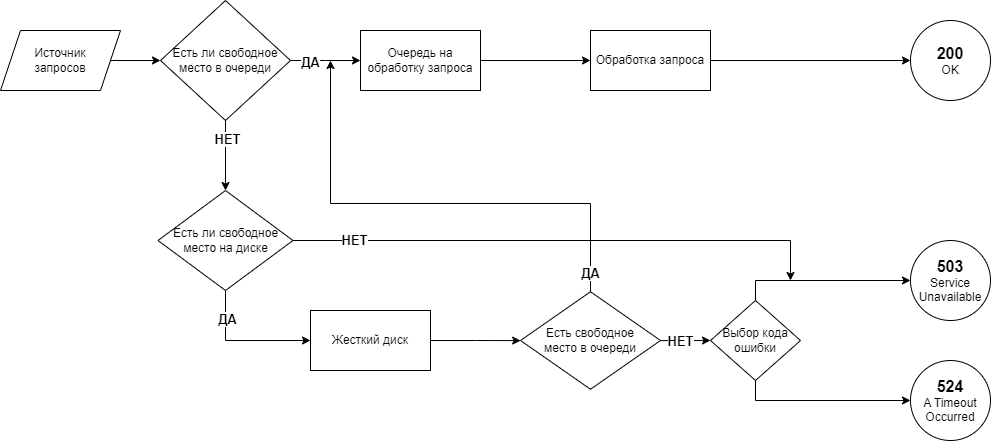
\includegraphics[width=0.9\linewidth]{concept.png}}
    \caption{Логическая блок--схема разработанной модели}
    \label{concept}
\end{figure}

Составляющие приведенной схемы представляют следующее:
\begin{itemize}
    \item Параллелограмм --- точка входа в модель системы. Представляет собой централизованное
    место прибытия новых запросов на сервер из различных источников.
    \item Ромб --- развилка, соответствует выбору или определению способа дальнейшей
    обработки запроса в зависимости от текущего состояния системы
    \item Прямоугольник --- определяет процессы, происходящие с поступившим запросом.
    В рамках составленной модели - обработка запроса или ожидание в очереди. 
    \item Круг --- конечные этапы жизненного цикла запроса в рамках созданной модели.
    Обозначают непосредственные результаты обработки запроса, успешные или нет.
\end{itemize}
\newpage

\section{Создание модели в среде AnyLogic}
\begin{figure} [h]
    \center{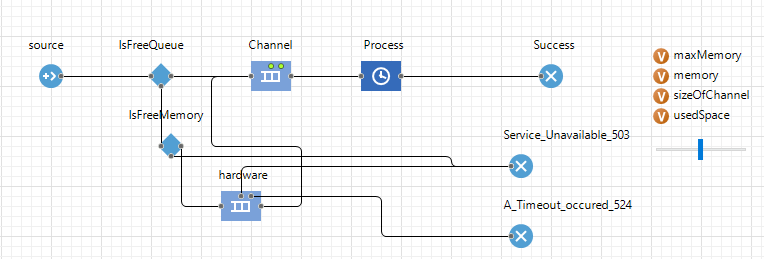
\includegraphics[width=0.9\linewidth]{model.png}}
    \caption{реализация разработанной модели DNS--сервера в среде AnyLogic}
\end{figure}


\subsection{Описание семантики элементов}
При построении дискретно--событийной модели применялись следующие
элементы палитры блока «Библиотека моделирования процессов» из стандартного
пакета AnyLogic \cite{anylogic}:
\begin{itemize}
    \item Source –-- тип блока, являющийся точкой входа модели. Предназначен для
    создания потока агентов. В данной модели представлен в виде единственного
    блока «start» для порождения агентов типа "Запрос".
    \item Queue –-- тип блока, реализующий очередь. Предназначен для управления
    потоком агента, формирования блока с входом и выходом типа FIFO. В
    данной модели используется дли имитирования очереди запросов на
    обработку в сервере ("Channel"), а также для имитации памяти и очереди на жестком
    диске (hardware).
    \item Delay –-- тип блока, реализующий временную задержку. Предназначен для
    приостановки хода движения агента. В данной модели представлен в виде
    блока "Process", которые содержат в себе семантику обработки запросов
    сервером.
    \item SelectOutput --- тип блока, реализующий логическое ветвление.
    Предназначен для ветвления хода движения агентов по вероятности или
    условию. Представлен в модели блоками "isFreeQueue" и "isFreeMemory".
    Первый реализует развилку по наличию свободного места в очереди запросов на сервер,
    а второй проверяет наличие свободной памяти на жестком диске.
    \item Sink –-- тип блока, являющийся точкой выхода модели. По нему можно
    отслеживать количество агентов, дошедших до конца. В данной модели
    представлен тремя блоками: "Success", "Service\_Unavaliable\_503" и
    "A\_Timeout\_Occured\_524", уничтожающими агентов. Первый отвечает за уход запроса из системы при его
    успешной обработке, второй за ситуацию, когда запросы переполняют по памяти жесткий диск и
    сервер ложится, и последний за случай, когда запрос пробыл на жестком диске больше времени, чем это
    допустимо условиями задачи.
\end{itemize}

\subsection{Описание логики элементов}
В представленной модели, внутри всех блоков реализована дополнительная логика поведения
с использованием языка программирования Java, в соответствии с предоставляемыми AnyLogic
возможностями.

Условия внедрены в соответствии с концептуальной моделью системы. Данные внедрения
позволяют динамически вычислять такие, необходимые для правильной работы параметры,
как:
\begin{itemize}
    \item Динамически изменять оставшееся место на диске в зависимости от количества
    пришедших и записанных на него запросов, а также реализовывать логику
    ошибок сервера 503 и 524, при невозможности или несвоевременности
    обработки запроса.
    \begin{figure} [h]
        \center{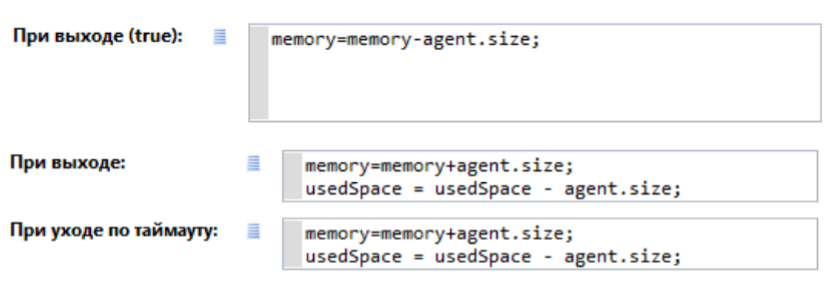
\includegraphics[width=0.9\linewidth]{entries.png}}
        \caption{Настройки связки блоков IsFreeMemory и hardware ---
        обрабатывающие выделение/высвобождение места на диске.}
    \end{figure}
    \item Ветвить условия для распределения запросов по циклам их обработки, в зависимости
    от текущего состояния и конфигурации системы.
    \begin{figure} [h]
        \center{
\includegraphics[width=0.9\linewidth]{branch.png}}
        \caption{Блок IsQueueFree --- отвечающий за отправку запроса в очередь
        на обработку либо же отправки на жесткий диск для ожидания.}
    \end{figure}

    \item Регулировать настройки системы во время ее работы, что является важным
    аспектом для проведения качественного исследования и определения наиболее оптимальных
    параметров, обозначенных в формулировке задачи. В данном случае регулируемыми
    параметрами являются:
    \begin{itemize}
        \item Скорость обработки запроса
        \item Максимально допустимый объем диска. Линейно зависит от скорости обработки
        запроса исходя из представленной в условии задачи формулы.
    \end{itemize}

    \begin{figure} [h]
        \center{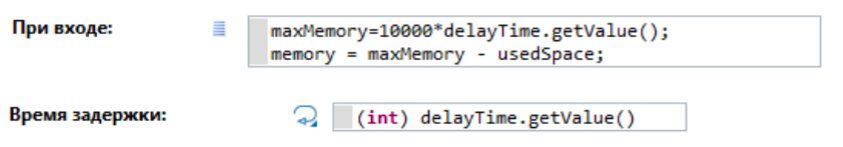
\includegraphics[width=0.9\linewidth]{mem.png}}
        \caption{Настройки связки блоков IsQueueFree и Process,
        представленные на рисунке настройки позволяют реализовать
        изменение параметров системы в динамике}
    \end{figure}

    \item Настройки ухода по тайм--ауту в блоке hardware а также условие в блоке
    IsFreeMemory реализуют логику ошибок обработки запроса на сервере. В случае
    ухода по тайм--ауту ошибка 524 A Timeout Occurred --- превышен лимит ожидания,
    в случае несрабатывания условия в блоке IsFreeMemory --- 503 Service Unavailable,
    что говорит о переполненном диске и невозможности серверу обработать запрос.

    \begin{figure} [h]
        \center{
\includegraphics[width=0.9\linewidth]{perm.png}}
        \caption{Настройки блоков hardware и IsFreeMemory соответственно}
    \end{figure}

    \item Динамически генерировать количество и размеры приходящих запросов. А
    именно длину, для определения занимаемого объема памяти на диске и интенсивность
    поступления запросов, что обеспечивает нелинейное поведение нагрузки на систему.
    \begin{figure} [h]
        \center{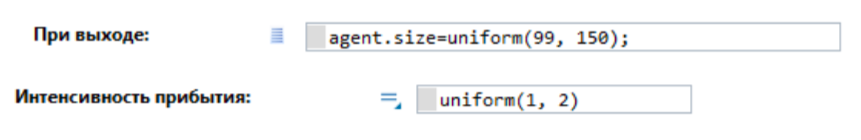
\includegraphics[width=0.9\linewidth]{source.png}}
        \caption{Настройки блока source, отвечающие за размер запроса, а именно,
        переменной size агента Запрос, а также случайную интенсивность поступления
        нагрузки соответственно.}
    \end{figure}
\end{itemize}

\newpage
\subsection{Вспомогательные элементы}
Для задания некоторых параметров модели и проведения экспериментов в модели использовались следующие вспомогательные элементы:
\begin{enumerate}
    \item Переменная \textit{maxMemory} --- переменная, необходимая для возможности динамически задавать максимальный размер жесткого диска (
    максимальный размер ЖД был сделан динамическим в целях упрощения проведения серий экспериментов, чтобы не приходилось задавать его вручную
    в зависимости от интенсивности, в момент проведения каждого эксперимента maxMemory является фиксированной величиной)
    \item Переменная \textit{memory} --- переменная, отражающая количество оставшегося места на диске с учетом пришедшего в него на очередь запроса.
    \item Переменная \textit{sizeOfChannel} --- переменная, описывающая искомую величину --- пропускную способность сервера.
    \item Переменная \textit{usedSpace} --- переменная, которая описывает занятое место на диске с учетом пришедшего запроса.
    \item Агент \textit{Запрос} --- транзакт, играющий роль запроса и содержащий информацию о размере этого запроса в байтах.
\end{enumerate}

\subsection{Элементы визуализации}
В качестве элементов визуализации используются три графика (рис. \ref{graphs}).

\begin{figure} [h]
    \center{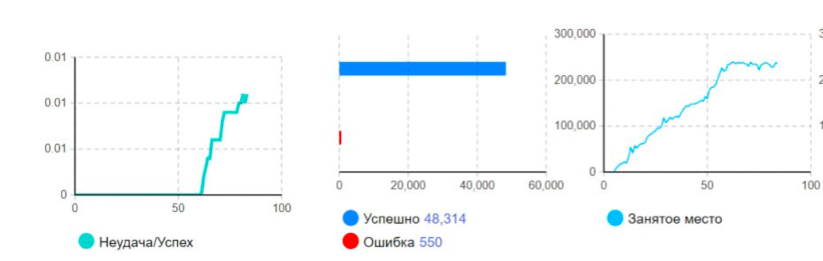
\includegraphics[width=0.9\linewidth]{graphs.png}}
    \caption{Пример графиков соотношения, динамики потребления памяти и количественных показателей сервера}
    \label{graphs}
\end{figure}

Первый отражает соотношение запросов которые не были
обработаны к числу успешно обработанных запросов, второй отражает динамику потребления памяти в зависимости от
времени, а третий показывает количество успешных и "провальных" запросов.

\newpage
\section{Имитационный эксперимент}
\subsection{Эксперименты}
По построенной модели проводились серии экспериментов. Было проведено по 4 эксперимента для
каждого времени суток: с высоким значением пропускной способности, с оптимальным значением
пропускной способности, с низким её значением и с экстремально низким значением. Для всех
экспериментов объем диска общий и равен 234,375 Мб (240 000 байт) и время обработки запроса С = 200 мс.
\begin{itemize}
    \item Утро
    \begin{enumerate}
        \item Интенсивность запросов --- uniform(100, 500), пропускная способность --- экстремально низкая:
        10 запросов (рис. \ref{mor1}).
        \begin{figure} [h]
            \center{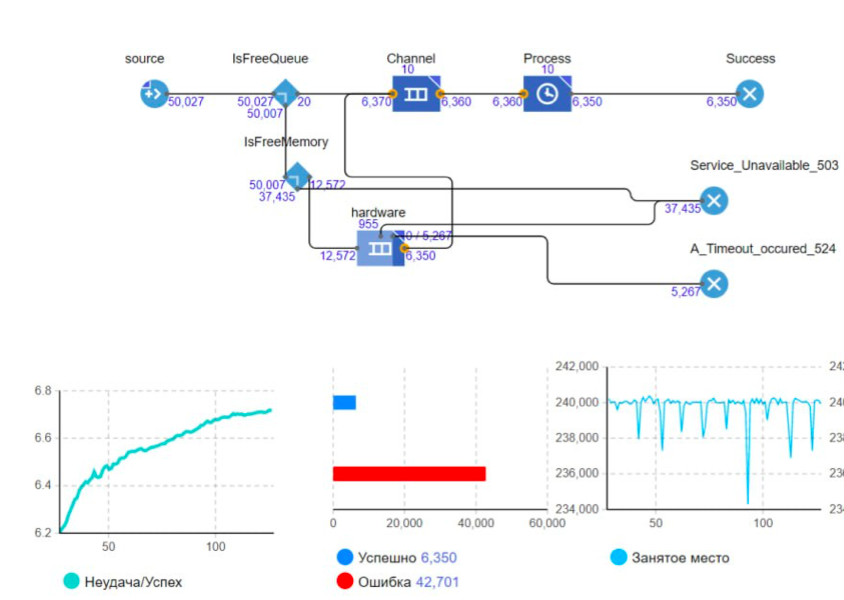
\includegraphics[width=0.6\linewidth]{mor1.png}}
            \caption{\textbf{Эксперимент 1:} утренний период, интенсивность uniform(100, 500), sizeOfChannel = 10}
            \label{mor1}
        \end{figure}
        \textbf{Результат:} пропускная способность слишком низкая при данной интенсивности,
        что ведет к переполнению жесткого диска и "вылету" из него запросов как по тайм--ауту, так и по памяти.
        Соотношение ошибок и успехов больше 1. 

        \item Интенсивность запросов та же --- uniform(100, 500), пропускная способность --- низкая: 60 запросов
        (рис. \ref{mor2}).
        \begin{figure} [h]
            \center{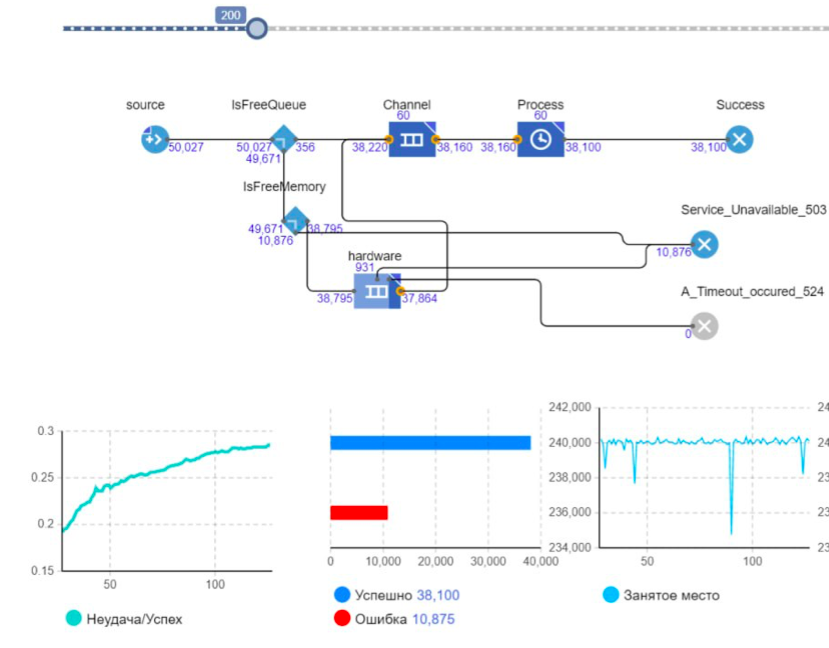
\includegraphics[width=0.6\linewidth]{mor2.png}}
            \caption{\textbf{Эксперимент 2:} утренний период, интенсивность uniform(100, 500), sizeOfChannel = 60}
            \label{mor2}
        \end{figure}
        \textbf{Результат:} пропускная способность все еще низкая при данной интенсивности, по--прежнему
        происходит переполнение диска по памяти, но уже в значительно меньшем количестве, а ошибок по
        тайм--ауту вообще не наблюдается. Соотношение успех/провал --- 28,5 процентов (неудовлетворительно).

        \item Интенсивность запросов та же --- uniform(100, 500), пропускная способность --- оптимальная:
        75 запросов (рис. \ref{mor3}).
        \begin{figure} [h]
            \center{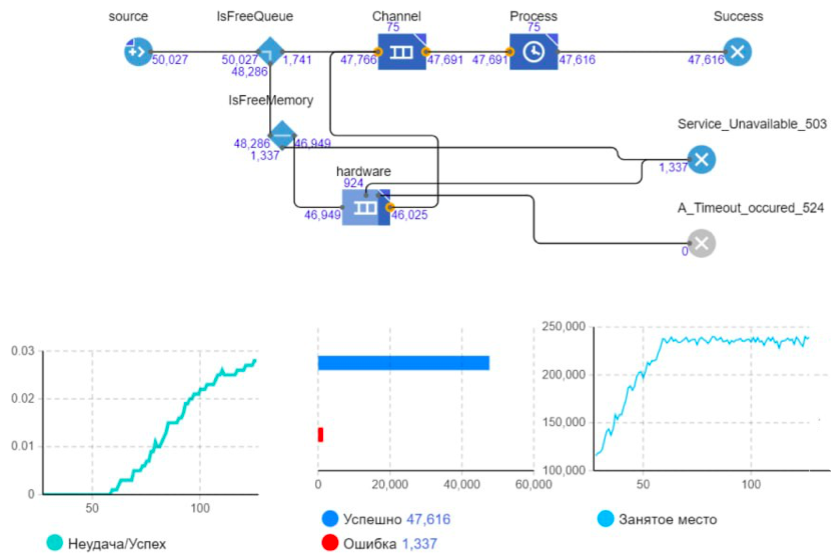
\includegraphics[width=0.6\linewidth]{mor3.png}}
            \caption{\textbf{Эксперимент 3:} утренний период, интенсивность uniform(100, 500), sizeOfChannel = 75}
            \label{mor3}
        \end{figure}
        \textbf{Результат:} пропускная способность оптимальна, на графике потребления
        памяти видно, что он не прижат постоянно вплотную к заданному лимиту памяти диска (происходят флуктуации)
        ошибок по тайм--ауту нет, а соотношение ошибок и успехов в высшей точке достигает примерно 3 процентов,
        что удовлетворительно.

        \newpage
        \item Интенсивность запросов та же --- uniform(100, 500), пропускная способность --- слишком высокая:
        171 запрос (рис. \ref{mor4}).
        \begin{figure} [h]
            \center{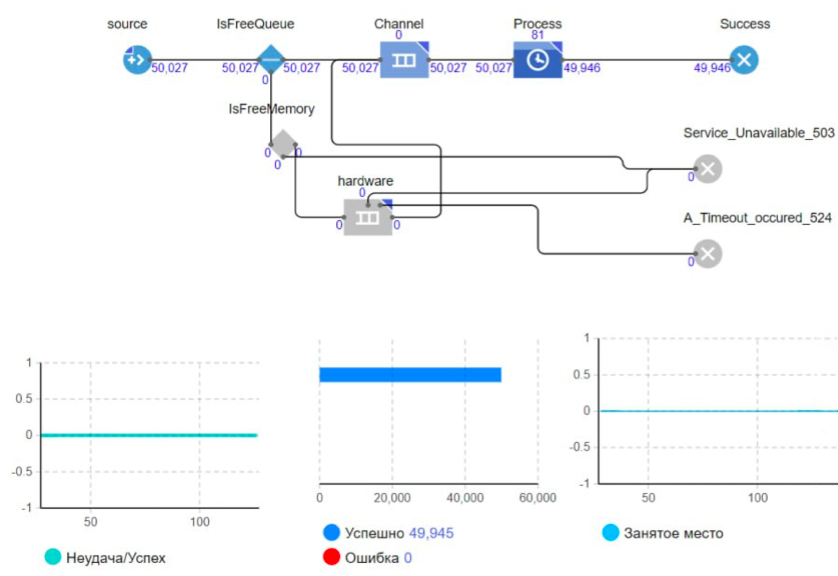
\includegraphics[width=0.6\linewidth]{mor4.png}}
            \caption{\textbf{Эксперимент 4:} утренний период, интенсивность uniform(100, 500), sizeOfChannel = 171}
            \label{mor4}
        \end{figure}
        \textbf{Результат:} пропускная способность слишком велика, ошибок не происходит вообще,
        а на жесткий диск запросы не попадают. Не удовлетворительно, поскольку тех же результатов 
        можно добиться с меньшей пропускной способностью.
    \end{enumerate}

    \item День: по сравнению с утром интенсивность запросов возрастает.
     \begin{enumerate}
        \item Интенсивность запросов --- uniform(500, 700), пропускная способность --- экстремально низкая:
        10 запросов (рис. \ref{aft1}).
        \begin{figure} [h]
            \center{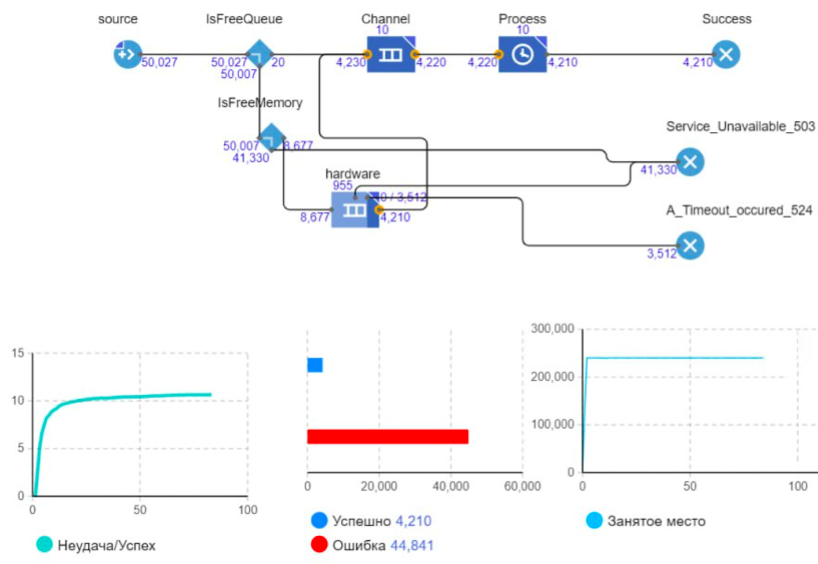
\includegraphics[width=0.6\linewidth]{aft1.png}}
            \caption{\textbf{Эксперимент 1:} дневной период, интенсивность uniform(500, 700), sizeOfChannel = 10}
            \label{aft1}
        \end{figure}
        \textbf{Результат:} пропускная способность слишком низкая при данной
        интенсивности, соотношение ошибок и успехов превышает 1, диск постоянно переполнен, большинство
        ошибок из--за переполнения памяти, ошибки по тайм--ауту также присутствуют. Не удовлетворительно.

        \newpage
        \item Интенсивность запросов та же --- uniform(500, 700), пропускная способность --- низкая:
        100 запросов (рис. \ref{aft2}).
        \begin{figure} [h]
            \center{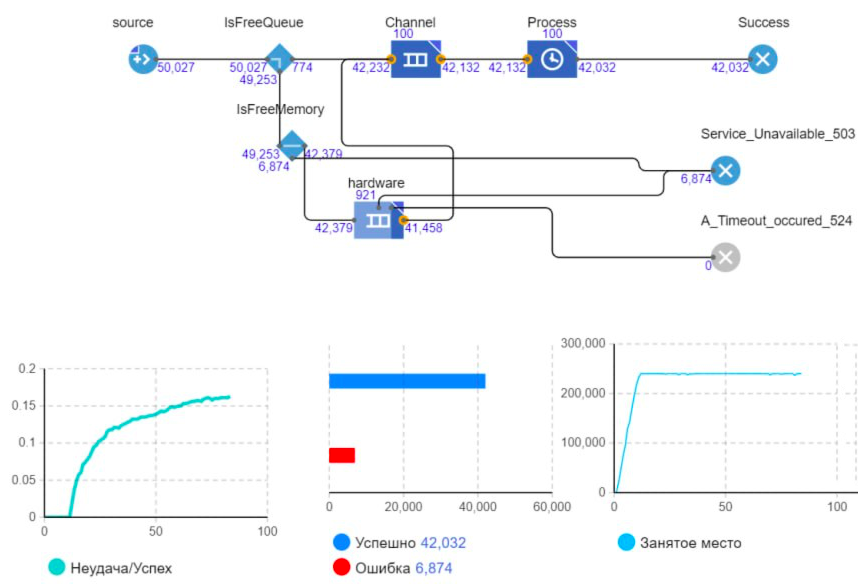
\includegraphics[width=0.6\linewidth]{aft2.png}}
            \caption{\textbf{Эксперимент 2:} дневной период, интенсивность uniform(500, 700), sizeOfChannel = 100}
            \label{aft2}
        \end{figure}
        \textbf{Результат:} пропускная способность все еще низкая,
        место на диске постоянно заполнено, ошибок по тайм--ауту уже нет, но по переполнению диска --- присутствуют.
        Соотношение успехов и ошибок --- примерно 17 процентов, что неудовлетворительно.

        \newpage
        \item Интенсивность запросов та же --- uniform(500, 700), пропускная способность --- оптимальная:
        115 запросов (рис. \ref{aft3}).
        \begin{figure} [h]
            \center{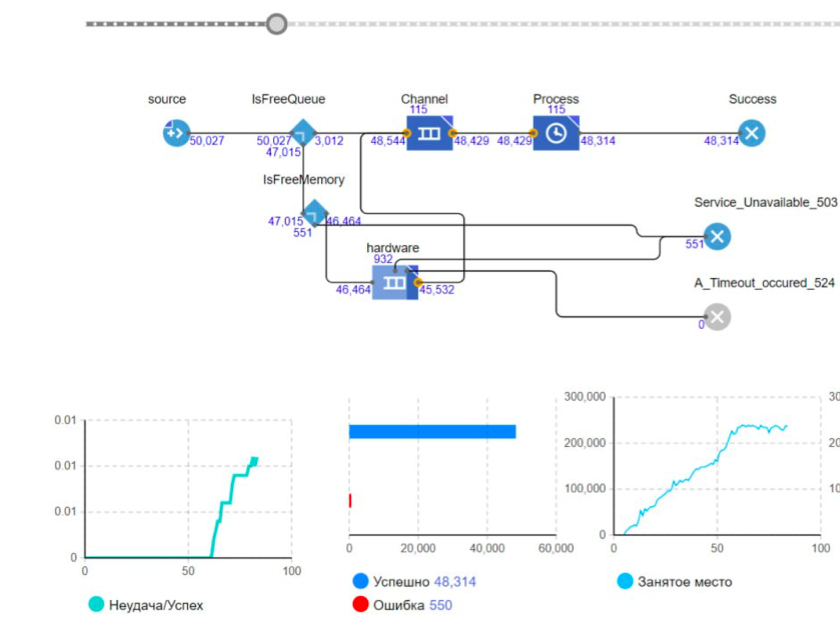
\includegraphics[width=0.6\linewidth]{aft3.png}}
            \caption{\textbf{Эксперимент 3:} дневной период, интенсивность uniform(500, 700), sizeOfChannel = 115}
            \label{aft3}
        \end{figure}
        \textbf{Результат:} пропускная способность оптимальна, после заполнения
        есть моменты когда диск немного освобождается, ошибок по тайм--ауту нет, соотношение ошибок и успехов ---
        в районе 1 процента. Результат удовлетворяет оптимальным условиям.

        \newpage
        \item Интенсивность запросов та же --- uniform(500, 700), пропускная способность --- слишком высокая:
        120 запросов (рис. \ref{aft4}).
        \begin{figure} [h]
            \center{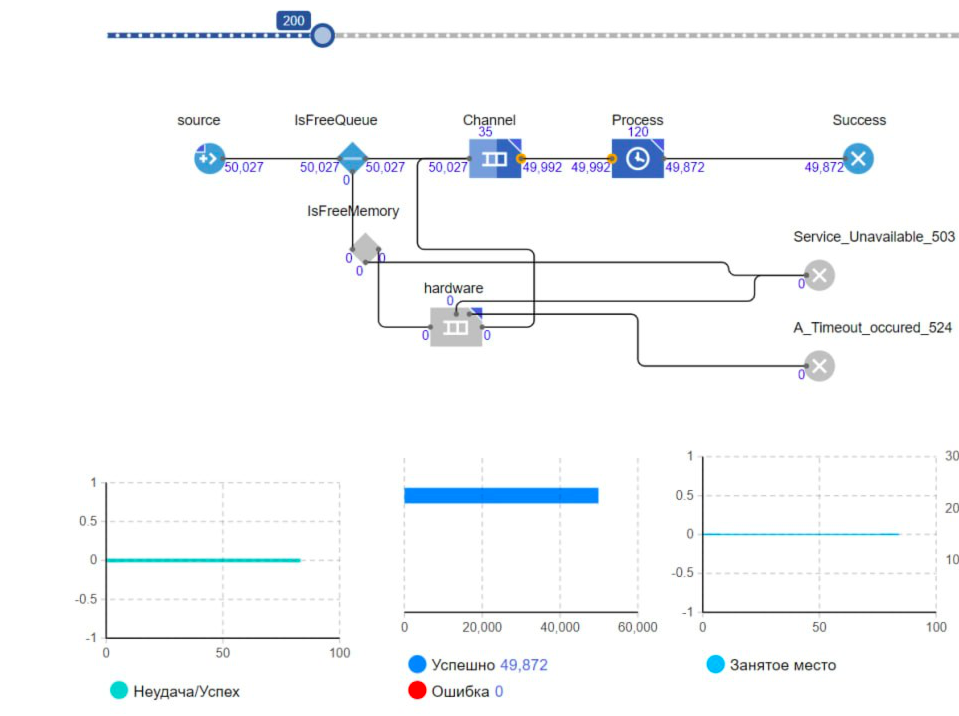
\includegraphics[width=0.6\linewidth]{aft4.png}}
            \caption{\textbf{Эксперимент 4:} дневной период, интенсивность uniform(500, 700), sizeOfChannel = 120}
            \label{aft4}
        \end{figure}
        \textbf{Результат:} пропускная способность слишком высока, место на диске совсем
        не используется, ошибок не происходит. Не удовлетворительно, поскольку примерно тех же результатов можно
        достичь с меньшей пропускной способностью.
    \end{enumerate}

    \item Вечер: максимальная интенсивность из всех трех периодов дня.
     \begin{enumerate}
        \item Интенсивность запросов --- uniform(700, 1000), пропускная способность --- экстремально низкая:
        10 запросов (рис. \ref{evn1}).
        \begin{figure} [h]
            \center{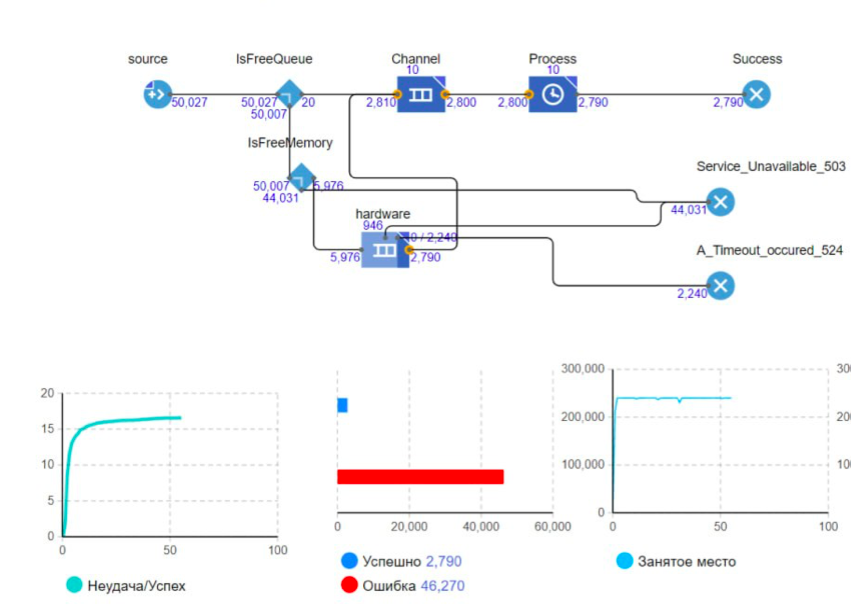
\includegraphics[width=0.6\linewidth]{evn1.png}}
            \caption{\textbf{Эксперимент 1:} вечерний период, интенсивность uniform(700, 1000), sizeOfChannel = 10}
            \label{evn1}
        \end{figure}
        \textbf{Результат:} пропускная способность слишком мала: присутствуют
        ошибки и по тайм--ауту и по переполнению диска, соотношение ошибок и успеха больше 1, место на диске
        постоянно занято. Неудовлетворительно.

        \item Интенсивность запросов --- uniform(700, 1000), пропускная способность --- низкая:
        120 запросов (рис. \ref{evn2}).
        \begin{figure} [h]
            \center{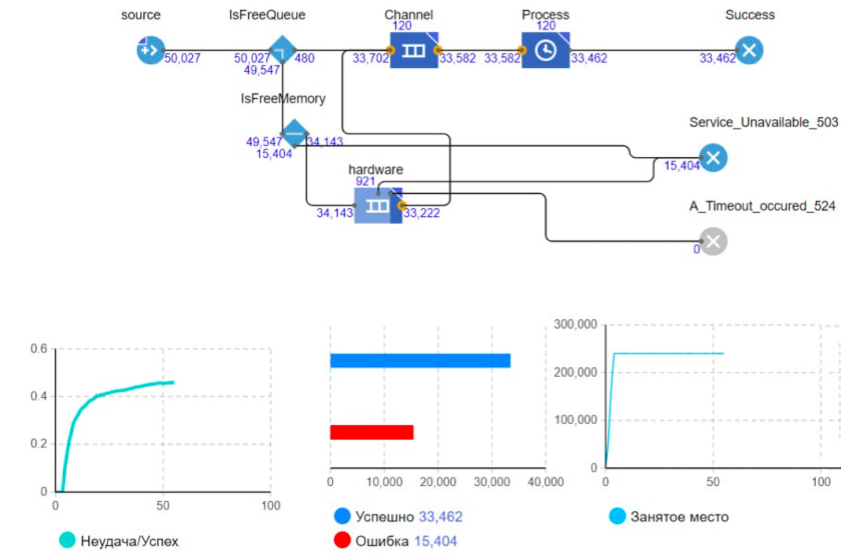
\includegraphics[width=0.6\linewidth]{evn2.png}}
            \caption{\textbf{Эксперимент 2:} вечерний период, интенсивность uniform(700, 1000), sizeOfChannel = 120}
            \label{evn2}
        \end{figure}
        \textbf{Результат:} пропускная способность все еще слишком низкая:
        ошибок по тайм--ауту уже нет, но соотношение успешных и ошибочных запросов примерно 50/50, что
        говорит о неоптимальности пропускной способности.
        \newpage

        \item Интенсивность запросов --- uniform(700, 1000), пропускная способность --- оптимальная:
        171 запрос (рис. \ref{evn3}).
        \begin{figure} [h]
            \center{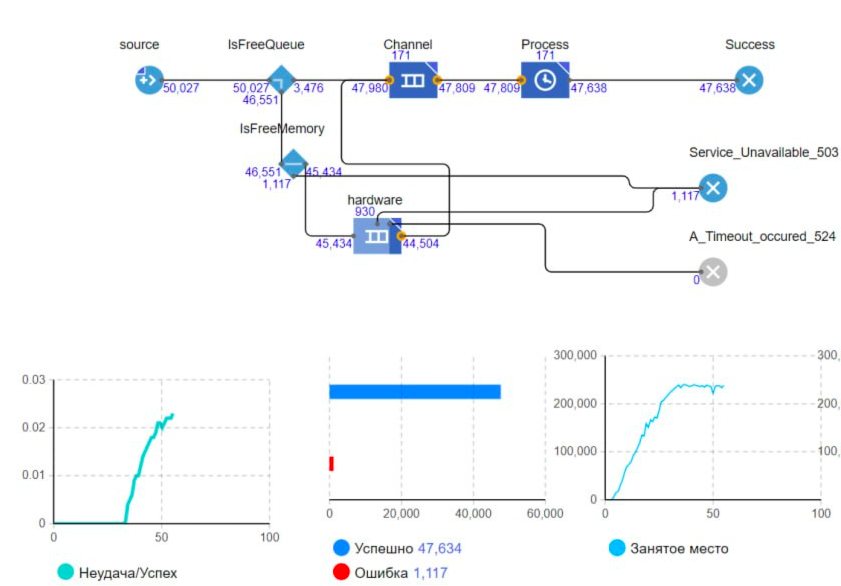
\includegraphics[width=0.6\linewidth]{evn3.png}}
            \caption{\textbf{Эксперимент 3:} вечерний период, интенсивность uniform(700, 1000), sizeOfChannel = 171}
            \label{evn3}
        \end{figure}
        \textbf{Результат:} пропускная способность оптимальная: диск не постоянно
        заполнен до предела (стабильные флуктуации), ошибок по тайм--ауту нет, а соотношение ошибок "по вылету"
        и успешных запросов чуть больше 2 процентов.
        \newpage
        \item Интенсивность запросов --- uniform(700, 1000), пропускная способность --- слишком высокая:
        180 запросов (рис. \ref{evn4}).
        \begin{figure} [h]
            \center{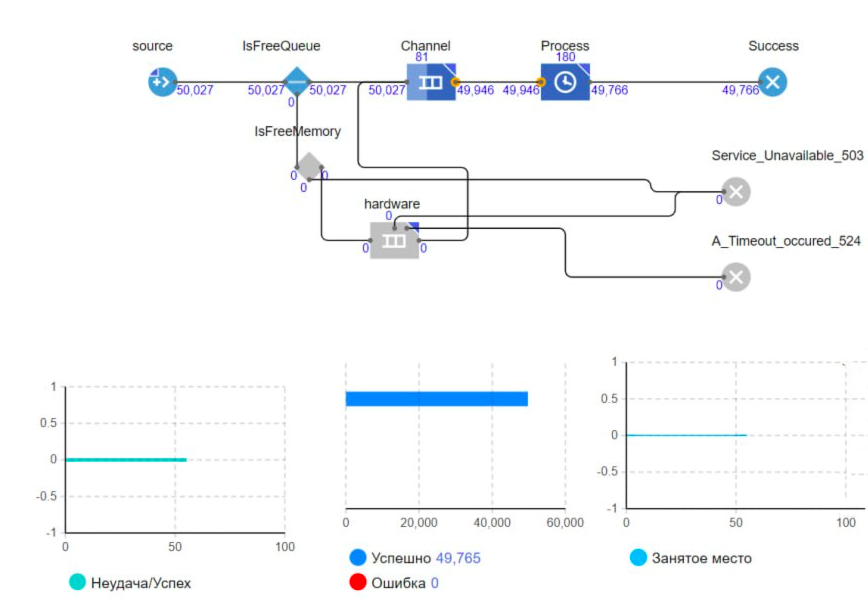
\includegraphics[width=0.6\linewidth]{evn4.png}}
            \caption{\textbf{Эксперимент 4:} вечерний период, интенсивность uniform(700, 1000), sizeOfChannel = 180}
            \label{evn4}
        \end{figure}
        \textbf{Результат:} пропускная способность слишком высокая, жесткий диск
        не используется, ошибок не наблюдается, значение не оптимально, поскольку значение пропускной способности
        можно сделать меньше без потери эффективности.

    \end{enumerate}
\end{itemize}

\subsection{Выводы}
Рассмотрим теперь результаты экспериментов. Они приведены в таблице \ref{tab1}. Из данной таблицы можно
сделать вывод что интенсивность запросов и пропускная способность коррелируют следующим образом: чем
выше интенсивность, тем выше должны быть пропускная способность.

\begin{table}[h]
    \begin{tabular}{|l|l|l|}
    \hline
    Время суток & Интенсивность (зап./сек)      & \begin{tabular}[c]{@{}l@{}}Оптимальное значение\\ интенсивности (запросов за раз)\end{tabular} \\ \hline
    Утро        & uniform(100, 500)  & 75                                                                                             \\ \hline
    День        & uniform(500, 700)  & 115                                                                                            \\ \hline
    Вечер       & uniform(700, 1000) & 171                                                                                            \\ \hline
    \end{tabular}
    \caption{Результаты подбора оптимальной пропускной способности в течение суток}
    \label{tab1}
\end{table}

\newpage
\section{Заключение}
В заключении можно сказать, что при выполнении данной работы была построена дискретно--событийная модель,
эмулирующая поведение DNS--сервера в разное время дня. Был проведен имитационный эксперимент, с целью сравнения
оптимального значения пропускной способности, требуемой интенсивностью в различное время суток.

По результатам эксперимента можно утверждать, что интенсивность и пропускная способность связаны так, что
чем больше одна, там больше другая. Таким образом если планируется делать сервер с большой интенсивностью
приходящих запросов, следует увеличить его пропускную мощность в обработке запросов.


\newpage
\begin{thebibliography}{}
    \bibitem{dns} Mao Z. M. et al. A Precise and Efficient Evaluation of the Proximity Between Web Clients and Their Local DNS Servers
    // USENIX Annual Technical Conference, General Track. – 2002. – С. 229-242.
    \bibitem{server} Cohen J. W. The single server queue. – Elsevier, 2012.
    \bibitem{fifo} Morse D., Richardson G. The LIFO/FIFO Decision // Journal of accounting research. – 1983. – С. 106-127.
    \bibitem{anylogic} Merkuryeva G., Bolshakovs V. Vehicle schedule simulation with AnyLogic
    // 2010 12th International Conference on Computer Modelling and Simulation. – IEEE, 2010. – С. 169-174.
\end{thebibliography}

\end{document}